\documentclass{beamer}
\usepackage[utf8]{inputenc}
\usetheme{Madrid}
\usecolortheme{default}
\usepackage{amsmath,amssymb,amsfonts,amsthm}
\usepackage{txfonts}
\usepackage{tkz-euclide}
\usepackage{listings}
\usepackage{adjustbox}
\usepackage{array}
\usepackage{tabularx}
\usepackage{gvv}
\usepackage{lmodern}
\usepackage{circuitikz}
\usepackage{tikz}
\usepackage{graphicx}
\setbeamertemplate{page number in head/foot}[totalframenumber]
\usepackage{tcolorbox}
\tcbuselibrary{minted,breakable,xparse,skins}
\definecolor{bg}{gray}{0.95}
\DeclareTCBListing{mintedbox}{O{}m!O{}}{%
breakable=true,
listing engine=minted,
listing only,
minted language=#2,
minted style=default,
minted options={%
linenos,
gobble=0,
breaklines=true,
breakafter=,,
fontsize=\small,
numbersep=8pt,
#1},
boxsep=0pt,
left skip=0pt,
right skip=0pt,
left=25pt,
right=0pt,
top=3pt,
bottom=3pt,
arc=5pt,
leftrule=0pt,
rightrule=0pt,
bottomrule=2pt,
toprule=2pt,
colback=bg,
colframe=orange!70,
enhanced,
overlay={%
\begin{tcbclipinterior}
\fill[orange!20!white] (frame.south west) rectangle ([xshift=20pt]frame.north west);
\end{tcbclipinterior}},
#3,
}
\lstset{
language=C,
basicstyle=\ttfamily\small,
keywordstyle=\color{blue},
stringstyle=\color{orange},
commentstyle=\color{green!60!black},
numbers=left,
numberstyle=\tiny\color{gray},
breaklines=true,
showstringspaces=false,
}


\title
{5.2.45}
\date{September 30, 2025}
\author
{EE25BTECH11043 - Nishid Khandagre}

\begin{document}

\frame{\titlepage}

\begin{frame}{Question}
Solve the system of linear equations:
\begin{align*}
x + 2y = 2\\
2x + 3y = 3
\end{align*}
\end{frame}

\begin{frame}{Theoretical Solution}
Given:
\begin{align}
x+2y&=2 \\
2x+3y&=3
\end{align}

\begin{align}
\myvec{1&2\\2&3}\myvec{x\\y}&=\myvec{2\\3}
\end{align}
\end{frame}

\begin{frame}{Theoretical Solution}
Write the augmented matrix:
\begin{align}
\myaugvec{2}
{1 & 2 & 2 \\
2 & 3 & 3}
\end{align}
Eliminate the first column using the operation $R_2 \to R_2 - 2R_1$:
\begin{align}
\myaugvec{2}
{1 & 2 & 2 \\
0 & -1 & -1}
\end{align}
\end{frame}

\begin{frame}{Theoretical Solution}
Next, apply the operation $R_2 \to -R_2$:
\begin{align}
\myaugvec{2}
{1 & 2 & 2 \\
0 & 1 & 1}
\end{align}
Then, apply $R_1 \to R_1 - 2R_2$
\begin{align}
\myaugvec{2}
{1 & 0 & 0 \\
0 & 1 & 1}
\end{align}
\end{frame}

\begin{frame}{Theoretical Solution}
\begin{align}
\myvec{x\\y}&=\myvec{0\\1}
\end{align}
Therefore, the solution to the system of linear equations is:
\begin{align}
x = 0 \\
y = 1
\end{align}
\end{frame}

\begin{frame}[fragile]
\frametitle{C Code}
\begin{lstlisting}
#include <stdio.h>

// Function to solve a 2x2 system of linear equations
// a1, b1, c1: coefficients for the first equation (a1x + b1y = c1)
// a2, b2, c2: coefficients for the second equation (a2x + b2y = c2)
// x_sol, y_sol: pointers to store the solutions for x and y
void solveLinearSystem(double a1, double b1, double c1,
                       double a2, double b2, double c2,
                       double *x_sol, double *y_sol) {
    double determinant = a1 * b2 - a2 * b1;

    *x_sol = (c1 * b2 - c2 * b1) / determinant;
    *y_sol = (a1 * c2 - a2 * c1) / determinant;
}
\end{lstlisting}
\end{frame}

\begin{frame}[fragile]
\frametitle{Python Code using C shared library}
\begin{lstlisting}
import ctypes
import numpy as np
import matplotlib.pyplot as plt

# Load the shared library
lib_solver = ctypes.CDLL("./code10.so")

# Define the argument types and return type for the C function
lib_solver.solveLinearSystem.argtypes = [
    ctypes.c_double,  # a1
    ctypes.c_double,  # b1
    ctypes.c_double,  # c1
    ctypes.c_double,  # a2
    ctypes.c_double,  # b2
    ctypes.c_double,  # c2
    ctypes.POINTER(ctypes.c_double), # x_sol
    ctypes.POINTER(ctypes.c_double)  # y_sol
]
\end{lstlisting}
\end{frame}

\begin{frame}[fragile]
\frametitle{Python Code using C shared library}
\begin{lstlisting}
lib_solver.solveLinearSystem.restype = None
# Given system of linear equations:
# x + 2y = 2
# 2x + 3y = 3
a1_given, b1_given, c1_given = 1.0, 2.0, 2.0
a2_given, b2_given, c2_given = 2.0, 3.0, 3.0

# Create ctypes doubles to hold the results
x_solution = ctypes.c_double()
y_solution = ctypes.c_double()

# Call the C function to solve the system
lib_solver.solveLinearSystem(
    a1_given, b1_given, c1_given,
    a2_given, b2_given, c2_given,
    ctypes.byref(x_solution),
    ctypes.byref(y_solution)
)
\end{lstlisting}
\end{frame}

\begin{frame}[fragile]
\frametitle{Python Code using C shared library}
\begin{lstlisting}
x_found = x_solution.value
y_found = y_solution.value

print(f"The solution to the system is: x = {x_found:.2f}, y = {y_found:.2f}")
# Optional: Plotting the lines to visualize the intersection
# Define a range for x values
x_vals = np.linspace(-5, 5, 400)

# Calculate y values for the first equation: y = (2 - x) / 2
y1_vals = (c1_given - a1_given * x_vals) / b1_given

# Calculate y values for the second equation: y = (3 - 2x) / 3
y2_vals = (c2_given - a2_given * x_vals) / b2_given
\end{lstlisting}
\end{frame}

\begin{frame}[fragile]
\frametitle{Python Code using C shared library}
\begin{lstlisting}
plt.figure(figsize=(8, 6))
plt.plot(x_vals, y1_vals, label=f'{a1_given}x + {b1_given}y = {c1_given}')
plt.plot(x_vals, y2_vals, label=f'{a2_given}x + {b2_given}y = {c2_given}')

# Plot the intersection point
plt.scatter(x_found, y_found, color='red', s=100, zorder=5, 
            label=f'Solution ({x_found:.2f}, {y_found:.2f})')
plt.annotate(f'({x_found:.2f},{y_found:.2f})', (x_found, y_found), 
             textcoords="offset points", xytext=(5,5), ha='left', color='red')
\end{lstlisting}
\end{frame}

\begin{frame}[fragile]
\frametitle{Python Code using C shared library}
\begin{lstlisting}
plt.xlabel('x')
plt.ylabel('y')
plt.title('Solution of Linear Equations (using C shared library)')
plt.grid(True)
plt.axhline(0, color='black', linewidth=0.5)
plt.axvline(0, color='black', linewidth=0.5)
plt.legend()
plt.savefig("fig1.png")
plt.show()
\end{lstlisting}
\end{frame}

\begin{frame}[fragile]
\frametitle{Pure Python Code}
\begin{lstlisting}
import numpy as np
import matplotlib.pyplot as plt

# Function to solve a 2x2 system of linear equations
def solve_2x2_system(a1, b1, c1, a2, b2, c2):
    det = a1 * b2 - a2 * b1
    if det == 0:
        return None, None # No unique solution
    x = (c1 * b2 - c2 * b1) / det
    y = (a1 * c2 - a2 * c1) / det
    return x, y

# Given equations
# x + 2y = 2
# 2x + 3y = 3
a1, b1, c1 = 1, 2, 2
a2, b2, c2 = 2, 3, 3
\end{lstlisting}
\end{frame}

\begin{frame}[fragile]
\frametitle{Pure Python Code}
\begin{lstlisting}
# Solve the system
x_solution, y_solution = solve_2x2_system(a1, b1, c1, a2, b2, c2)

if x_solution is not None and y_solution is not None:
    print(f"Solution: x = {x_solution}, y = {y_solution}")

    # Generate points for plotting the lines
    x_vals = np.linspace(-5, 5, 400)

    # First equation: x + 2y = 2  => y = (2 - x) / 2
    y1_vals = (2 - x_vals) / 2

    # Second equation: 2x + 3y = 3 => y = (3 - 2x) / 3
    y2_vals = (3 - 2 * x_vals) / 3
\end{lstlisting}
\end{frame}

\begin{frame}[fragile]
\frametitle{Pure Python Code Cont.}
\begin{lstlisting}[language=Python]
    # Plotting
    plt.figure(figsize=(8, 6))
    plt.plot(x_vals, y1_vals, label='x + 2y = 2')
    plt.plot(x_vals, y2_vals, label='2x + 3y = 3')

    # Plot the intersection point
    plt.plot(x_solution, y_solution, 'ro', markersize=8, 
             label=f'Solution: ({x_solution:.2f}, {y_solution:.2f})')
    plt.annotate(f'({x_solution:.2f}, {y_solution:.2f})', (x_solution, y_solution),
                 textcoords="offset points", xytext=(10,10), ha='center')

    plt.xlabel('x')
    plt.ylabel('y')
    plt.title('Solution of a System of Linear Equations (Pure Python)')
    \end{lstlisting}
\end{frame}

\begin{frame}[fragile]
\frametitle{Pure Python Code}
\begin{lstlisting}
    plt.axhline(0, color='gray', linestyle='--', linewidth=0.7)
    plt.axvline(0, color='gray', linestyle='--', linewidth=0.7)
    plt.grid(True)
    plt.legend()
    plt.axis('equal') # Ensures equal scaling for x and y axes
    plt.xlim(-5, 5)
    plt.ylim(-5, 5)
    plt.savefig("fig2.png")
    plt.show()

    print("Figure saved as fig2.png")

else:
    print("The system has no unique solution (lines are parallel or coincident)")
\end{lstlisting}
\end{frame}

\begin{frame}{Plot by Python using shared output from C}
\begin{figure}[H]
\centering
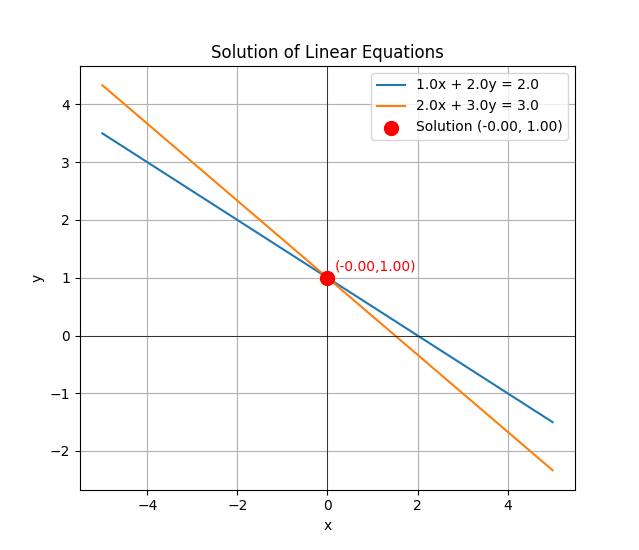
\includegraphics[width=0.8\columnwidth]{../figs/fig1.png}
\caption{}
\label{fig:1}
\end{figure}
\end{frame}
 
\begin{frame}{Plot by Python only}
\begin{figure}[H]
\centering
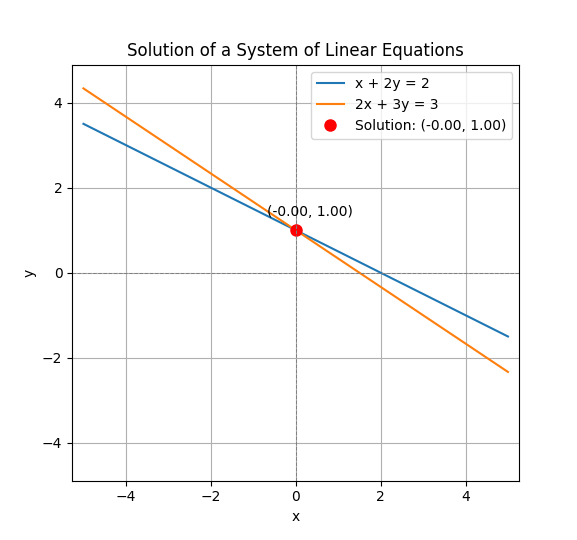
\includegraphics[width=0.7\columnwidth]{../figs/fig2.png}
\caption{}
\label{fig:2}
\end{figure}
\end{frame}

\end{document}
